\documentclass[oneside,final,14pt,a4paper]{extreport}

\usepackage{tempora}   

\usepackage{vmargin}
\setpapersize{A4}
\setmarginsrb{2.5cm}{2.2cm}{2.2cm}{2.2cm}{0pt}{10mm}{0pt}{13mm}
\usepackage{setspace}
\sloppy
\setstretch{1.5}
\usepackage{indentfirst}
\parindent=1.25cm

%%%%% ADDED TO SUPPORT TT BOLD FACES %%%%
\DeclareFontShape{OT1}{cmtt}{bx}{n}{<5><6><7><8><9><10><10.95><12><14.4><17.28><20.74><24.88>cmttb10}{}
\renewcommand{\ttdefault}{pcr}
%%%%% END %%%%%%%%%%%%%%%%%%%%%%%%%%%%%%% 
\usepackage{atbegshi,picture}
\usepackage[T1,T2A]{fontenc} 
\usepackage[utf8]{inputenc}
\usepackage[main=russian,english]{babel}
\usepackage[backend=biber,style=ieee,autocite=inline]{biblatex}
\bibliography{ref.bib}
\usepackage{csquotes}
\usepackage{blindtext}


\usepackage{pdfpages}
\newenvironment{bottompar}{\par\vspace*{\fill}}{\clearpage}

% \usepackage{cite}
\usepackage{amsmath,amsfonts}
\usepackage{amsthm}
\newtheorem{theorem}{Theorem}
\newtheorem{corollary}{Corollary}
\newtheorem{lemma}{Lemma}
\newtheorem{proposition}{Proposition}
\theoremstyle{definition}
\newtheorem{definition}{Definition}
\theoremstyle{remark}
\newtheorem*{remark}{Remark}
\theoremstyle{remark}
\newtheorem*{example}{Example}



\usepackage{graphicx}
\graphicspath{{figs/}} %path to images
\usepackage{multirow,array}
\usepackage{caption}
\usepackage{subcaption}
\usepackage[unicode]{hyperref}
\hypersetup{colorlinks=true, linkcolor=black, citecolor=black}
\usepackage{paralist}
\usepackage{listings}
\usepackage{zed-csp}
\usepackage{fancyhdr}
\usepackage{color,colortbl}
\usepackage{booktabs}
\usepackage{epsfig} % for postscript graphics files

\usepackage{upgreek} 
\usepackage{bm}
\usepackage{hyperref}
\usepackage{longtable}
\usepackage[font=singlespacing, labelfont=bf]{caption}
\usepackage{floatrow}

\pagestyle{fancyplain}

\definecolor{commentgreen}{RGB}{2,112,10}
\definecolor{eminence}{RGB}{108,48,130}
\definecolor{weborange}{RGB}{255,165,0}
\definecolor{frenchplum}{RGB}{129,20,83}

\lstdefinelanguage{elixir}{
    morekeywords={case,catch,def,do,else,false,%
        use,alias,receive,timeout,defmacro,defp,%
        for,if,import,defmodule,defprotocol,%
        nil,defmacrop,defoverridable,defimpl,%
        super,fn,raise,true,try,end,with,%
        unless},
    otherkeywords={<-,->, |>, \%\{, \}, \{, \, (, )},
    sensitive=true,
    morecomment=[l]{\#},
    morecomment=[n]{/*}{*/},
    morecomment=[s][\color{purple}]{:}{\ },
    morestring=[s][\color{orange}]"",
    commentstyle=\color{commentgreen},
    keywordstyle=\color{eminence},
    stringstyle=\color{red},
	showstringspaces=false,
  captionpos=b
}

\definecolor{verylightgray}{rgb}{.97,.97,.97}


\lstdefinelanguage{solidity}{
	keywords=[1]{anonymous, assembly, assert, balance, break, call, callcode, case, catch, class, constant, continue, constructor, contract, debugger, default, delegatecall, delete, do, else, emit, event, experimental, export, external, false, finally, for, function, gas, if, implements, import, in, indexed, instanceof, interface, internal, is, length, library, log0, log1, log2, log3, log4, memory, modifier, new, payable, pragma, private, protected, public, pure, push, require, return, returns, revert, selfdestruct, send, solidity, storage, struct, suicide, super, switch, then, this, throw, transfer, true, try, typeof, using, value, view, while, with, addmod, ecrecover, keccak256, mulmod, ripemd160, sha256, sha3}, % generic keywords including crypto operations
	keywordstyle=[1]\color{blue}\bfseries,
	keywords=[2]{address, bool, byte, bytes, bytes1, bytes2, bytes3, bytes4, bytes5, bytes6, bytes7, bytes8, bytes9, bytes10, bytes11, bytes12, bytes13, bytes14, bytes15, bytes16, bytes17, bytes18, bytes19, bytes20, bytes21, bytes22, bytes23, bytes24, bytes25, bytes26, bytes27, bytes28, bytes29, bytes30, bytes31, bytes32, enum, int, int8, int16, int24, int32, int40, int48, int56, int64, int72, int80, int88, int96, int104, int112, int120, int128, int136, int144, int152, int160, int168, int176, int184, int192, int200, int208, int216, int224, int232, int240, int248, int256, mapping, string, uint, uint8, uint16, uint24, uint32, uint40, uint48, uint56, uint64, uint72, uint80, uint88, uint96, uint104, uint112, uint120, uint128, uint136, uint144, uint152, uint160, uint168, uint176, uint184, uint192, uint200, uint208, uint216, uint224, uint232, uint240, uint248, uint256, var, void, ether, finney, szabo, wei, days, hours, minutes, seconds, weeks, years},	% types; money and time units
	keywordstyle=[2]\color{teal}\bfseries,
	keywords=[3]{block, blockhash, coinbase, difficulty, gaslimit, number, timestamp, msg, data, gas, sender, sig, value, now, tx, gasprice, origin},	% environment variables
	keywordstyle=[3]\color{violet}\bfseries,
	identifierstyle=\color{black},
	sensitive=true,
	comment=[l]{//},
	morecomment=[s]{/*}{*/},
	commentstyle=\color{gray},
	stringstyle=\color{red},
	morestring=[b]',
  captionpos=b,
	morestring=[b]"
}

\lstdefinelanguage{yul}{
  keywords={let, function, if, else, switch, case, default, for, break, continue, return, true, false},
  keywordstyle=\color{blue}\bfseries,
  ndkeywords={add, sub, mul, div, sdiv, mod, smod, addmod, mulmod, exp, signextend, lt, mstore8, mstore},
  ndkeywordstyle=\color{teal}\bfseries,
  comment=[l]{//},
  morecomment=[s]{/*}{*/},
  commentstyle=\color{gray},
  stringstyle=\color{red},
  morestring=[b]",
  morestring=[b]',
  sensitive=true,
  numbers=left,
  % numberstyle=\tiny\color{gray},
  stepnumber=1,
  numbersep=10pt,
  tabsize=4,
  showspaces=false,
  showstringspaces=false,
  showtabs=false,
  % frame=single,
  captionpos=b,
  breaklines=true,
  breakatwhitespace=false,
  escapeinside={\%*}{*)}
}

\definecolor{delim}{RGB}{20,105,176}
\colorlet{numb}{magenta!60!black}
\colorlet{punct}{red!60!black}

\lstdefinelanguage{json}{
    numbers=left,
    numberstyle=\scriptsize,
    stepnumber=1,
    numbersep=8pt,
    showstringspaces=false,
    breaklines=true,
    frame=lines,
    literate=
     *{0}{{{\color{numb}0}}}{1}
      {1}{{{\color{numb}1}}}{1}
      {2}{{{\color{numb}2}}}{1}
      {3}{{{\color{numb}3}}}{1}
      {4}{{{\color{numb}4}}}{1}
      {5}{{{\color{numb}5}}}{1}
      {6}{{{\color{numb}6}}}{1}
      {7}{{{\color{numb}7}}}{1}
      {8}{{{\color{numb}8}}}{1}
      {9}{{{\color{numb}9}}}{1}
      {:}{{{\color{punct}{:}}}}{1}
      {,}{{{\color{punct}{,}}}}{1}
      {\{}{{{\color{delim}{\{}}}}{1}
      {\}}{{{\color{delim}{\}}}}}{1}
      {[}{{{\color{delim}{[}}}}{1}
      {]}{{{\color{delim}{]}}}}{1},
}

\lstset{numbers=left,xleftmargin=2em,frame=single,framexleftmargin=0em,numberstyle=\footnotesize\ttfamily}

\lstset{
	language=yul,
	backgroundcolor=\color{verylightgray},
	extendedchars=true,
	basicstyle=\footnotesize\ttfamily,
	showstringspaces=false,
	showspaces=false,
	numbers=left,
	numberstyle=\footnotesize,
	numbersep=9pt,
	tabsize=2,
	breaklines=true,
	showtabs=false,
	captionpos=b
}


% remember section title
\renewcommand{\chaptermark}[1]%
	{\markboth{\chaptername~\thechapter~--~#1}{}}

% subsection number and title
\renewcommand{\sectionmark}[1]%
	{\markright{\thesection\ #1}}

\rhead[\fancyplain{}{\bf\leftmark}]%
      {\fancyplain{}{\bf\thepage}}
\lhead[\fancyplain{}{\bf\thepage}]%
      {\fancyplain{}{\bf\rightmark}}
\cfoot{} %bfseries


\newcommand{\dedication}[1]
   {\thispagestyle{empty}
     
   \begin{flushleft}\raggedleft #1\end{flushleft}
}

\hypersetup{colorlinks=true, allcolors=black, citecolor=black}


\begin{document}


\includepdf[offset=1in -1in,noautoscale, pages=-]{title_annotation.pdf}

\newpage
\tableofcontents
\begin{abstract}
% skip one line to make the abstract start with indent

Моя аннотация начинается здесь.
\end{abstract}
\setcounter{page}{4}
% set manually the number, from which Глава 1 starts!
% Why do we put 4 in this case?
% Title page - page 1
% Оглавление - page 2
% Аннотация - page 3
% Глава 1 - page 4
% In your annotation the counter number can be different, please count carefully and insert the corresponding number.

\chapter{Введение}
\label{chap:intro}

\section{Спрос на новый язык}
\label{sec:langdemand}

Разработчики dApp в основном используют язык программирования Solidity. Моноязычность и монопарадигматизм ограничивают гибкость и креативность разработчиков. Кроме того, высокий порог вхождения, связанный с этим языком, может отпугнуть новичков. Для овладения им часто требуются значительные затраты времени и сил, что замедляет процесс разработки.

Учитывая эти ограничения, существует возможность для создания нового языка. Функциональная альтернатива, особенно та, которая поддерживает динамическую типизацию и опирается на основы общепризнанного языка программирования, могла бы значительно повысить доступность и эффективность разработки dApp. Такой язык не только облегчит освоение новым разработчикам, но и откроет новые возможности для инноваций в пространстве Web3. Такой потенциал делает разработку нового языка перспективным направлением для расширения возможностей и охвата среды программирования Ethereum.

\section{Цель работы}
\label{sec:goal}

\subsection{Цели и гипотезы исследования}
Нашей целью является создание языка смарт-контрактов с синтаксисом Elixir и динамическими типами - Elixireum. В результате язык должен быть выразительным, по крайней мере, чтобы иметь возможность реализовать токены ERC-20\footnote{https://eips.ethereum.org/EIPS/eip-20} и ERC-721\footnote{https://eips.ethereum.org/EIPS/eip-721}. Мы планировали добавить такие возможности, как неизменяемость, поддержка макросов и сопостовление с образцом, чтобы сделать этот язык функциональным. Также мы ожидали, что Elixireum будет потреблять столько же или меньше газа по сравнению с Solidity.

\subsection{Ожидаемые результаты}
\begin{itemize}
  \item \textbf{Рабочий компилятор для Elixireum:} Разработка компилятора, способного транслировать язык Elixireum в байткод EVM.
  
  \item \textbf{Развернутый токен ERC-20:} Развернутый токен ERC-20, написанный на Elixireum, в качестве демонстрации того, что Elixireum обладает фундаментальной функциональностью, необходимой для разработки смарт-контрактов.
  
  \item \textbf{Сравнительное потребление газа:} Анализ потребления газа для контрактов Elixireum и сравнительная оценка с Solidity.
\end{itemize}
% \chapter{Literature Review}
\label{chap:lr}
\chaptermark{Second Chapter Heading}


\section{Ethereum Virtual Machine}
Ethereum is a decentralized system, and at its core, the Ethereum Virtual Machine (EVM) is an essential component of the Ethereum blockchain. The EVM serves as the computational heart of the Ethereum network, enabling the execution of smart contracts and providing the foundation for a wide array of decentralized applications.

In the context of smart contract execution, it's important to mention the concept of gas limit. Gas limit is a critical aspect of Ethereum's execution model. Each operation and computation on the Ethereum Virtual Machine consumes a certain amount of gas, which is a measure of computational work. The gas limit is a cap set by the user or the entity initiating a contract execution, and it represents the maximum amount of gas they are willing to spend for that operation.

Gas limit, the EVM's stack-based architecture, and the wide set of available operations allow it to efficiently and securely for miners execute these smart contracts, granting it the status of a Turing-complete machine \cite{EthereumWhitepaper}. This level of computational flexibility empowers developers to create sophisticated programs.

\section{Existing EVM languages}
According to the official Ethereum documentation \cite{OfficialEthereumLanguages} only four languages for EVM exist: Solidity, Vyper, Yul and Fe. However, other attempts to create language for EVM are known \cite{CommunityEthereumLanguages}. Although there are many EVM languages, according to sOmEtHiNg only two of them are widely used: Solidity and Vyper.

\subsection{Solidity}

\subsection{Vyper}

\section{Market Research}

\section{Elixir}

\section{Compiler construction}

\section{Conclusion}

% \newpage


% \begin{longtable}{c|c}
% \caption[This is the title I want to appear in the List of Tables]{Simulation Parameters} \label{table:secsimulation_params} \\
% \hline
% A & B  \\
% \hline
% \endfirsthead
% \multicolumn{2}{@{}l}{} \\
% \hline
% A & B \\
% \hline
% \endhead
% \hline
%  \textbf{Parameter} & \textbf{Value}\\
%  \hline
%  Number of vehicles & $|\mathcal{V}|$\\
%  \hline
%  Number of RSUs & $|\mathcal{U}|$\\
%  \hline
%  RSU coverage radius & 150 m\\
%  \hline
%  V2V communication radius & 30 m\\
%  \hline
%  Smart vehicle antenna height & 1.5 m\\
%  \hline
%  RSU antenna height & 25 m\\
%  \hline
%  Smart vehicle maximum speed & $v_{max}$ m/s\\
%  \hline
%  Smart vehicle minimum speed & $v_{min}$ m/s\\
%  \hline
%  Common smart vehicle cache capacities & $[50, 100, 150, 200, 250]$ mb\\
%  \hline
%  Common RSU cache capacities & $[5000,1000,1500,2000,2500]$ mb\\
%  \hline
%  Common backhaul rates & $[75, 100, 150]$ mb/s\\
%  \hline
% \end{longtable}

% \begin{figure}[hbt]
% \centering
% 
\includegraphics[]{figs/inno.png}
% \caption{One kernel at $x_s$ (\emph{dotted kernel}) or two kernels at
% $x_i$ and $x_j$ (\textit{left and right}) lead to the same summed estimate
% at $x_s$. This shows a figure consisting of different types of
% lines. Elements of the figure described in the caption should be set in
% italics, in parentheses, as shown in this sample caption.}
% \label{fig:secex}
% \end{figure}

% This description implies several essential properties of the task at hand:
% \begin{enumerate}
%     \item Watermark must contain all necessary information, but still, be placeable and recognizable even on smaller images. The produced watermark must be compact but have the possibility to store enough information. 
%     \item To prevent easy tampering, the watermark must be invisible to the naked eye (and, preferably, to basic image parsing tools). If malefactor does not know about the existence of watermark, they might not even try to remove it and disable it. 
% \end{enumerate}

\chapter{Methodology}
\label{chap:met}
\chaptermark{Third Chapter Heading}

Chapter overview

\section{Compilers and evm theory}
\label{}

\subsection{Introduction to compilers}

Compiler construction is a sophisticated field in computer science, involving the creation of software that translates source code written in a high-level programming language into a lower-level language, often machine code. The process of compiler construction is typically divided into several distinct phases, each with its specialized function:


\begin{enumerate}
    \item Lexical Analysis
          \begin{itemize}
              \item Token Generation: The compiler's first phase involves breaking down the source code into tokens, which are the basic building blocks of the language (like keywords, operators, identifiers, literals).
              \item Regular Expressions: Lexical analyzers often use regular expressions to recognize these tokens, simplifying the source code into a stream of tokens for further processing.
          \end{itemize}

    \item Syntax Analysis
          \begin{itemize}
              \item Parsing: This phase involves analyzing the token sequence from lexical analysis to ensure that the expressions and statements conform to the rules of the programming language's grammar.
              \item Syntax Trees: The result is often a syntax tree, which represents the syntactic structure of the source code in a hierarchical tree format.
          \end{itemize}
    \item Semantic Analysis
          \begin{itemize}
              \item Type Checking: The compiler checks whether the parsed code makes logical sense, adhering to the language's semantic rules. This includes type checking, where the compiler verifies that each operation is compatible with its operands.
              \item Symbol Table: The compiler uses a symbol table to keep track of variable names, their types, and other relevant information to ensure correct interpretation and context.
          \end{itemize}
    \item Intermediate Code Generation
          \begin{itemize}
              \item Abstract Representation: The compiler translates the source code into an intermediate representation, which is a lower-level representation of the program that retains its logical structure.
              \item Platform-Independent Code: This intermediate code is typically platform-independent, serving as a bridge between the high-level source code and the machine code.
          \end{itemize}
    \item Optimization
          \begin{itemize}
              \item Performance Improvement: The optimization phase refines the intermediate code to improve efficiency and performance. This can include eliminating redundant calculations, optimizing loops, and more.
              \item Target-Dependent Optimizations: These optimizations often vary depending on the target machine's architecture and capabilities.
          \end{itemize}
    \item Code Generation
          \begin{itemize}
              \item Machine Code: The final phase involves translating the optimized intermediate code into machine code specific to the target machine CPU architecture or virtual machine instruction set.
              \item Assembly Language: Sometimes, the output is in the form of assembly language, which is then further translated into machine code by an assembler.
          \end{itemize}
    \item  Linking and Loading
          \begin{itemize}
              \item Linking: If the program consists of multiple source code files or external libraries, the linking process combines these into a single executable.
              \item Loading: The loader then places the executable into memory for execution by the machine.
          \end{itemize}
\end{enumerate}

In the context of Elixireum, these compiler construction principles must be adapted to suit the specific needs of the Ethereum Virtual Machine (EVM). This includes considerations for smart contract compilation, optimization for gas efficiency, and adhering to the deterministic execution model of the EVM. Understanding these compiler construction phases is essential for Elixireum development, as each stage plays a critical role in transforming high-level Elixireum code into efficient, secure, and EVM-compatible bytecode.

\subsection{Ethereum Virtual Machine - A Deeper Insight}

EVM is a core component of the Ethereum blockchain, pivotal in maintaining its decentralized and secure nature. It serves as an execution environment for smart contracts, enabling the remarkable functionality that Ethereum offers. Understanding the EVM is crucial for developing Elixireum, as it provides the foundational framework within which this new language operates.

\begin{enumerate}
    \item  Execution Environment
          \begin{itemize}
              \item Isolated System: The EVM operates as an isolated environment, completely sandboxed from the Ethereum network. This isolation ensures that code execution within the EVM does not directly affect the network or the filesystem of the host computer.
              \item Deterministic Execution: The EVM is designed to be deterministic. This means that executing the same smart contract with the same input will always produce the same output across all nodes in the Ethereum network. This characteristic is essential for maintaining consistency and agreement (consensus) across the decentralized network.
          \end{itemize}
    \item EVM's Role in Smart Contracts
          \begin{itemize}
              \item Smart Contract Lifecycle: Developers write smart contracts in high-level languages like Solidity or Vyper. These contracts are then compiled into EVM bytecode. When a contract is deployed on the Ethereum blockchain, it's executed by the EVM to ensure it behaves as expected.
              \item           Gas Mechanism: The EVM uses a gas mechanism to measure and limit the resources (computation and storage) a contract can use. Each operation in the EVM has a gas cost associated with it, preventing inefficient or malicious code from overloading the network.
          \end{itemize}
    \item State Machine
          \begin{itemize}
              \item           State Transitions: The EVM can be viewed as a state machine, where transactions transition the Ethereum blockchain from one state to another. Smart contracts, through their executions, modify the state stored in the Ethereum blockchain.
              \item           EVM Bytecode: The EVM interprets a series of bytes (bytecode) which instruct the machine on the operations to perform. This bytecode is the compiled version of high-level contract code.
          \end{itemize}
    \item Storage and Memory
          \begin{itemize}
              \item   Storage: The EVM has a long-term storage model, where data is stored persistently on the blockchain. This storage is expensive but necessary for maintaining the state across transactions.
              \item         Memory: The EVM also includes a volatile memory space, cleared after each transaction, used for temporary storage during contract execution.
          \end{itemize}
    \item Challenges and Considerations for Elixireum
          \begin{itemize}
              \item Gas Optimization: Given the cost implications of EVM operations, Elixireum must focus on gas optimization during the compilation process.
              \item Security and Determinism: Security vulnerabilities in smart contracts can be costly. Hence, Elixireum needs to ensure robust security measures. Additionally, the deterministic nature of the EVM requires that Elixireum-generated bytecode behaves consistently across all executions.
          \end{itemize}



\end{enumerate}




\section{Problems (no researches, more hacking way to research)}
\label{}

\section{Research design (methods: techonology stack, compiler stages, decisions like why we compile and not interpret)}
\label{}

\section{Limitations (elixirish distribution is not applicable to evm, so it is cannot be used in smart contracts, libraries are out of the scope, external smart contract interactions, need to spec types for public functions, need of solidity compiler )}
\label{}

\section{architecture and modules overview}
\label{}

\section{other languages comparison}
\label{}

\section{Conclusion}



\ldots

Referencing other chapters \ref{chap:lr}, \ref{chap:met}, \ref{chap:impl}, \ref{chap:eval} and \ref{chap:conclusion}
\begin{longtable}{c|c}
    \caption[This is the title I want to appear in the List of Tables]{Simulation Parameters} \label{table:thisimulation_params} \\
    \hline
    A                                     & B                                                                                    \\
    \hline
    \endfirsthead
    \multicolumn{2}{@{}l}{}                                                                                                      \\
    \hline
    A                                     & B                                                                                    \\
    \hline
    \endhead
    \hline
    \textbf{Parameter}                    & \textbf{Value}                                                                       \\
    \hline
    Number of vehicles                    & $|\mathcal{V}|$                                                                      \\
    \hline
    Number of RSUs                        & $|\mathcal{U}|$                                                                      \\
    \hline
    RSU coverage radius                   & 150 m                                                                                \\
    \hline
    V2V communication radius              & 30 m                                                                                 \\
    \hline
    Smart vehicle antenna height          & 1.5 m                                                                                \\
    \hline
    RSU antenna height                    & 25 m                                                                                 \\
    \hline
    Smart vehicle maximum speed           & $v_{max}$ m/s                                                                        \\
    \hline
    Smart vehicle minimum speed           & $v_{min}$ m/s                                                                        \\
    \hline
    Common smart vehicle cache capacities & $[50, 100, 150, 200, 250]$ mb                                                        \\
    \hline
    Common RSU cache capacities           & $[5000,1000,1500,2000,2500]$ mb                                                      \\
    \hline
    Common backhaul rates                 & $[75, 100, 150]$ mb/s                                                                \\
    \hline
\end{longtable}

\begin{figure}[hbt]
    \centering
    
\includegraphics[]{figs/inno.png}
    \caption{One kernel at $x_s$ (\emph{dotted kernel}) or two kernels at
        $x_i$ and $x_j$ (\textit{left and right}) lead to the same summed estimate
        at $x_s$. This shows a figure consisting of different types of
        lines. Elements of the figure described in the caption should be set in
        italics, in parentheses, as shown in this sample caption.}
    \label{fig:thiex}
\end{figure}


\ldots
\chapter{Design and Implementation}
\label{chap:impl}

% preliminary structure:

% 1. architecture
% 2. technical details (memory included)
% 3. modules details


% overview of architecture (.exm -> lexer -> parser -> compiler (code gen) -> .yul code -> solidity compiler -> EVM bytecode)
%                                                            |
%                                                            -> ABI generator

% detailed overview of modules (for example: calldata parsing, compiler (two passes), return data transformer, storage)


% technical details:
%   - memory organization
%     - how variables are stored, dynamic typing
%     - immutability of variables
%     - offset
%   - show events/module args syntax
%   - key features
%     - events
%     - constructor
%     - storage
%     - ABI for public functions
%     - reverts with utf-8 error string
%   - standard functions declaration on demand (transitivity included) and mechanism itself (module responsible for )

This chapter outlines the principal elements of the design of Elixireum compiler. It overviews the technology stack employed in the development process and underscores the pivotal decisions that shaped the architecture of the compiler.


\section{Stack overview}
\label{sec:architecture}
This section rationalize the technology stack used in the project: Elixir, Yul, Solidity compiler.
% TODO: add clarification that Elixir is base of the syntax and source language of the compiler
\subsection{Choice of Elixir}
Here is the rationalization behind the choice of Elixir:
\begin{itemize}
    \item One of the most popular open source blockchain explorers, Blockscout\footnote{\href{https://www.blockscout.com/}{https://www.blockscout.com} -- Official Blockscout website}, is written in Elixir. From this we can say that Elixir is well heard of in Web3 community.
    \item Our team possesses substantial expertise in this programming language.
    \item Elixir is open source so we can easily reuse its machinery for tokenization and parsing Elixireum.
\end{itemize}

\subsection{Choice of Yul}
\begin{itemize}
    \item Initially, our strategy was to compile Elixireum directly into EVM bytecode. Subsequently, we pivoted towards an intermediate representation (IR), selecting Yul as IR aligned with our requirements. Advantages from this decision are as follows:
        \begin{itemize}
            \item Compatibility with all EVM versions, eliminating the need for version-specific concerns. 
            \item Avoidance of reimplementing primitives such as function calls, variable and stack management, thereby freeing up resources to enhance the feature set of the language.
            \item Reduced gas consumption facilitated by the optimizer of Solidity compiler.
        \end{itemize}
      Despite these considerations, the choice comes with slight limitations, notably:
        \begin{itemize}
            \item Dependency on the Solidity compiler for Elixireum.
            \item The unresolved bug\footnote{\href{https://github.com/ethereum/solidity/issues?q=is:issue+is:open+StackTooDeepError}{https://github.com/ethereum/solidity/issues?q=is:issue+is:open+StackTooDeepError}} in the Solidity compiler, in our case it appears for large Elixireum smart contracts when compiled with the optimizer disabled. The bug results in an inability to operate with a large number of variables and deep stack depths.
        \end{itemize}
      No significant downsides compared to direct compilation to EVM bytecode.

    \item We also considered mapping BEAM (Erlang VM), target of Elixir, bytecode to EVM bytecode. However, this option presented significant challenges due to the fundamental architectural and philosophical differences between the two virtual machines. BEAM is specifically tailored for environments that demand high concurrency, distribution, and fault tolerance, and it includes a set of opcodes optimized for these conditions. In contrast, the EVM is designed to run smart contracts within blockchain ecosystems, prioritizing deterministic execution and gas metering to protect against spam and enhance network security. BEAM incorporates specialized instructions for concurrency and distributed processing that do not directly translate to the EVM, because of these distinct focuses.
\end{itemize}

\section{Technical details}

\subsection{Memory organization}
\label{sec:memory_organization}

In our language implementation, we decided to store all the runtime variables in the volatile memory of the EVM. This decision is justified by the low gas cost associated with the memory operations and the simplicity of implementation. We considered two alternatives: the transient storage, which is more expensive than memory, and the stack, which involves more complex management.

In the generated Yul code, a variable is defined as a pointer to the memory location where its value is stored. At this pointer, the first byte is reserved for the type number, and the subsequent bytes contain the value itself for simple cases. For more complex cases, such as lists and tuples, the first byte still indicates the type, followed by a word\footnote{in this context word is 32 bytes} that specifies the count of elements, and then the elements themselves, each stored as an inline variable (type + value). For strings or byte arrays, the first byte indicates the type (1 for strings, 102 for byte arrays), the next word specifies the byte count, followed by the actual bytes.

Since we developed a functional language, we should follow one of its fundamental principles -- immutability. This means that each assignment operation creates a new variable. In practice, we "forget" the previous pointer, assign a new pointer, and place the variable in a new location. Each new variable should be stored sequentially after the previous one. To achieve this, we define the offset\$ variable in the generated Yul code. This variable holds the memory address where the next variable will be stored. As a workaround for corner cases, we update this variable using the msize Yul function, assigning the current memory size rounded to one word to the offset\$ variable.

In Elixireum syntax, there are no type specifiers for variables. To handle dynamic types, we established several principles upon which our type system is built:
\begin{itemize}
  \item Return values of public functions must strictly match the specified types; otherwise, a revert\footnote{opcode which stops the current execution and throw an error. All the state changes are reverted} operation will be triggered.
  \item For literals, the type is defined at compile time.
  \item The type is stored in the first byte of the variable.
  \item We defined a standard cast function that developers can use in Elixireum code.

  The following code snippet demonstrates the usage of the cast function:
  \begin{lstlisting}[caption={Example of cast function usage}, language=elixir, label={lst:contract_structure}]
    @spec decimals() :: Types.UInt8.t()
    def decimals() do
      Utils.cast(18, Types.UInt8)
    end  
  \end{lstlisting}
\end{itemize}

The following Elixireum code illustrates a simple variable declaration:

\begin{lstlisting}[caption={Elixireum code for simple case}, language=elixir]
  a = 1
  b = 2
\end{lstlisting}

This Elixireum code is translated into Yul code as follows:

\begin{lstlisting}[caption={Generated yul code for simple case}, language=yul]
  let offset$ := msize()      // define offset$, set it to current memory size 
  let a$ := offset$           // define variable as the memory pointer
  mstore8(offset$, 67)        // 67 is int256 type, store it as one byte
  offset$ := add(offset$, 1)  // increase current offset by 1 byte, which is used by type on the line above
  mstore(offset$, 1)          // store the value itself
  offset$ := add(offset$, 32) // int256 value takes 32 bytes

  let b$ := offset$           // define variable as the memory pointer
  mstore8(offset$, 67)        // 67 is uin256 type
  offset$ := add(offset$, 1)  // increase current offset by 1 byte, which is used by type on the line above
  mstore(offset$, 2)          // store the value itself
  offset$ := add(offset$, 32) // int256 value takes 32 bytes
\end{lstlisting}

In this Yul code, offset\$ is initialized to the current memory size. Each variable (a\$ and b\$) is defined as a memory pointer. The type of each variable is stored using mstore8 Yul function, and the actual value is stored using mstore Yul function. The offset is incremented appropriately to account for the type byte and the 32-byte value for each variable.

The following table shows a snippet of the EVM memory for this simple case:

\begin{table}[h!]
  \centering
  \renewcommand{\arraystretch}{1.2} % Reduces the height of the table
  \begin{tabular}{|>{\centering\arraybackslash}m{2cm}|>{\centering\arraybackslash}m{1cm}|>{\centering\arraybackslash}m{1cm}|>{\centering\arraybackslash}m{1cm}|>{\centering\arraybackslash}m{0.75cm}|>{\centering\arraybackslash}m{1cm}|>{\centering\arraybackslash}m{1cm}|>{\centering\arraybackslash}m{1cm}|>{\centering\arraybackslash}m{1cm}|>{\centering\arraybackslash}m{0.75cm}|>{\centering\arraybackslash}m{1cm}|}
  \hline
  \textbf{Addresses} & 0x00 & 0x01 & 0x02 & ... & 0x21 & 0x22 & 0x23 & 0x24 & ... & 0x42 \\ \hline
  \textbf{Values}    & 0x43 & 0x00 & 0x00 & ... & 0x01 & 0x43 & 0x00 & 0x00 & ... & 0x01 \\ \hline
  \end{tabular}
  \caption{EVM Memory snippet for simple case}
  \label{tab:evm_memory}
  \end{table}

An example of handling strings in Elixireum is as follows:

\begin{lstlisting}[caption={Elixireum code for string case}, language=elixir]
  a = "abc" # hex representation of this utf-8 string is 0x616263
\end{lstlisting}
  
The corresponding Yul code generated for this string case is:

\begin{lstlisting}[caption={Generated yul code for string case}, language=yul]
  let offset$ := msize()      // define offset$, set it to current memory size 
  let a$ := offset$           // define variable as the memory pointer
  mstore8(offset$, 1)         // store the type, 1 is the string type
  offset$ := add(offset$, 1)  // increase current offset by 1 byte, which is used by type on the line above
  mstore(offset$, 3)          // store the byte size of the string
  offset$ := add(offset$, 32) // increase current memory pointer by 32 bytes, since the size of the string is 256 bit lenght
  mstore(offset$, 0x6162630000000000000000000000000000000000000000000000000000000000) \\ store the string itself
  offset$ := add(offset$, 3)  // string has length only 3 bytes
\end{lstlisting}

In this Yul code, the variable a\$ is defined as a memory pointer. The type of the variable is stored using mstore8, followed by storing the byte size of the string using mstore. The offset is incremented by the size of the string (3 bytes) after storing the string itself.

The following table illustrates a snippet of the EVM memory for this string case:

\begin{table}[h!]
  \centering
  \renewcommand{\arraystretch}{1.2} % Reduces the height of the table
  \begin{tabular}{|>{\centering\arraybackslash}m{2cm}|>{\centering\arraybackslash}m{1cm}|>{\centering\arraybackslash}m{1cm}|>{\centering\arraybackslash}m{1cm}|>{\centering\arraybackslash}m{0.75cm}|>{\centering\arraybackslash}m{1cm}|>{\centering\arraybackslash}m{1cm}|>{\centering\arraybackslash}m{1cm}|>{\centering\arraybackslash}m{1cm}|}
  \hline
  \textbf{Addresses} & 0x00 & 0x01 & 0x02 & ... & 0x20 & 0x21 & 0x22 & 0x23 \\ \hline
  \textbf{Values}    & 0x01 & 0x00 & 0x00 & ... & 0x03 & 0x61 & 0x62 & 0x63 \\ \hline
  \end{tabular}
  \caption{EVM Memory snippet for string case}
  \label{tab:evm_memory}
  \end{table}

An example of handling lists in Elixireum is as follows:

\begin{lstlisting}[caption={Elixireum code for list case}, language=elixir]
  a = [1, true, "abc"]
\end{lstlisting}
  
\begin{lstlisting}[caption={Generated yul code for string case}, language=yul]
  let offset$ := msize()
  
  // define int256 literal
  let var0$ := offset$
  ...  
  // define bool literal
  let bool_var1$ := offset$
  ...
  // define string literal
  let str2$ := offset$
  ...
  
  // define the list itself
  let a$ := offset$ // define variable as the memory pointer
  mstore8(offset$, 103) // store the list type
  offset$ := add(offset$, 1)
  mstore(offset$, 3) // store the length of the list 
  offset$ := add(offset$, 32) // increase current memory pointer by 32 bytes, since the size of the list is 256 bit lenght
  let ignored_
  ignored_, offset$ := copy_from_pointer_to$(var0$, offset$) // copy int256 variable to the start of the list & update offset$
  ignored_, offset$ := copy_from_pointer_to$(bool_var1$, offset$) // copy bool variable to the list & update offset$
  ignored_, offset$ := copy_from_pointer_to$(str2$, offset$) // copy string variable to the list & update offset$
\end{lstlisting}

In this Yul code the variables var0\$, bool\_var1\$, and str2\$ are defined for the integer, boolean, and string literals, respectively. Then list a\$ is defined. The length of the list is stored using mstore, and the actual values of the list elements are copied into memory using the copy\_from\_pointer\_to\$, function from Elixireum internal standard library (refer to implementation in Appendix \ref{appex:copy_from_pointer_to}), which updates the offset accordingly.

The following table illustrates a snippet of the EVM memory for this list case:
\begin{table}[h!]
  \centering
  \renewcommand{\arraystretch}{1.2} % Reduces the height of the table
  \begin{tabular}{|>{\centering\arraybackslash}m{3cm}|>{\centering\arraybackslash}m{1cm}|>{\centering\arraybackslash}m{1cm}|>{\centering\arraybackslash}m{1cm}|>{\centering\arraybackslash}m{1cm}|>{\centering\arraybackslash}m{1cm}|>{\centering\arraybackslash}m{1cm}|>{\centering\arraybackslash}m{1cm}|>{\centering\arraybackslash}m{1cm}|>{\centering\arraybackslash}m{1cm}|>{\centering\arraybackslash}m{1cm}|}
  \hline
  \textbf{Addresses} & ... & 0x47 & 0x48 & ... & 0x67 & 0x68 & 0x69 & ... & 0x88 & 0x89 \\ \hline
  \textbf{Values}    & ... & 0x67 & 0x00 & ... & 0x03 & 0x43 & 0x00 & ... & 0x01 & 0x02 \\ \hline \hline
  \textbf{Addresses} & 0x8a & 0x8b & 0x8c & ... & 0xab & 0xac & 0xad & 0xae & ... & ... \\ \hline
  \textbf{Values}    & 0x01 & 0x01 & 0x00 & ... & 0x03 & 0x61 & 0x62 & 0x63 & ... & ... \\ \hline
  \end{tabular}
  \caption{EVM Memory snippet for list case}
  \label{tab:evm_memory_aux} 
  \end{table}

\subsection{Key features}
\label{sec:key_features}

\begin{enumerate}
  \item \textbf{Events\footnote{\url{https://docs.soliditylang.org/en/v0.8.25/abi-spec.html\#events}}}

  Events are essential for highlighting storage changes or other significant events in the lifecycle of a smart contract. They can be easily retrieved from the blockchain after being emitted. Events can be defined and emitted in Elixireum as follows:

  \begin{lstlisting}[caption={Events}, language=elixir, label={lst:calldata_decoding_recursive}]
  @test name: "Test", indexed_arguments: [addr: Types.Address.t()], data_arguments: [value: Types.UInt256.t()]
    ...
  addr = ~ADDRESS(0x0000000000000000000000000000000000000000)
  value = 100
  Event.emit(@test, [addr: addr value: value])
  \end{lstlisting}
  
  \item \textbf{Storage}
  
  Each address in Ethereum has its own associated persistent storage, which functions as a key-value store with 32-byte keys and values. This storage is crucial for maintaining a global state. In Elixireum, storage variables can be specified as a module argument using the @ symbol. The type of the storage variable can be any available type, a mapping, or an inner mapping of any depth.

  \begin{lstlisting}[caption={Storage}, language=elixir, label={lst:calldata_decoding_recursive}]
    @balances type: %{Types.Address.t() => Types.UInt256.t()}
    @totalSupply type: Types.UInt256.t()
    ...
    Storage.store(@totalSupply, 1_000_000) # store the value to the storage
    supple = Storage.get(@totalSupply)     # get the value from the storage
    
    addr_1 = ... # define some address
    Storage.store(@balances[addr_1], 1_000)  # update the @balances mapping for addr_1
    balance = Storage.get(@balances[addr_1]) # get value for addr_1 from @balances
  \end{lstlisting}
  
  \item \textbf{Constructor}

  The constructor is called once, during the deployment of the smart contract. It is used to initialize the contract, set the owner, or define any other storage variables. Essentially, it executes any necessary operations upon contract creation.
  
  \begin{lstlisting}[caption={Constructor}, language=elixir, label={lst:calldata_decoding_recursive}]
    @spec constructor(Types.String.t(), Types.String.t()) :: nil
    def constructor(name, symbol) do
      Storage.store(@name, name)
      Storage.store(@symbol, symbol)
      Storage.store(@owner, Blockchain.caller())
    end
  \end{lstlisting}
  
  \item \textbf{Application Binary Interface (ABI) for Public Functions}
  
  The compiler enforces the specification of all public functions through compile-time errors. After compilation, all defined specifications are converted to the ABI JSON, which is necessary for correctly calling the smart contract after deployment.

  \begin{lstlisting}[caption={@spec}, language=elixir, label={lst:calldata_decoding_recursive}]
  @spec a(Types.Int256.t()) :: Types.String.t()
  def a(_int) do
    "return string"
  end
  \end{lstlisting}
  
  Resulting JSON ABI:
  \begin{lstlisting}[caption={ABI }, language=json, label={lst:calldata_decoding_recursive}]
    [
      {
          "name": "a",
          "type": "function",
          "outputs": [
              {
                  "name": "output",
                  "type": "string",
                  "internal_type": "string"
              }
          ],
          "inputs": [
              {
                  "name": "_int",
                  "type": "int256",
                  "internal_type": "int256"
              }
          ],
          "stateMutability": "view"
      }
  ]
  \end{lstlisting}
  
  \item \textbf{Reverts with UTF-8 Error String}

  Developers can revert the execution of a smart contract, optionally specify an error string. The revert reason for the transaction will be a hex-encoded UTF-8 string.

  \begin{lstlisting}[caption={Reverts}, language=elixir, label={lst:calldata_decoding_recursive}]
    raise "ERC20InvalidSender(address(0))"
  \end{lstlisting}
\end{enumerate}

\section{Modules overview}
This section provides a detailed overview of the main modules of the compiler. The modules are listed in the order corresponding to the contract life cycle i.e., deployment and then calls.
\subsection{Yul compiler}
The Yul compiler calls the Solidity compiler to generate bytecode, given the path to the standard JSON input file\footnote{\url{https://docs.soliditylang.org/en/v0.8.25/using-the-compiler.html\#input-description}}. For this purpose, it looks for the Solidity compiler that is capable of compiling Yul to bytecode. If there is no Solidity compiler already downloaded, the Yul compiler module downloads platform specific Solidity compiler. Then, it returns standard JSON output\footnote{\url{https://docs.soliditylang.org/en/v0.8.25/using-the-compiler.html\#output-description}}.
\subsection{Compiler}
\label{ssec:compiler}


\begin{figure}[H]
  \centering
  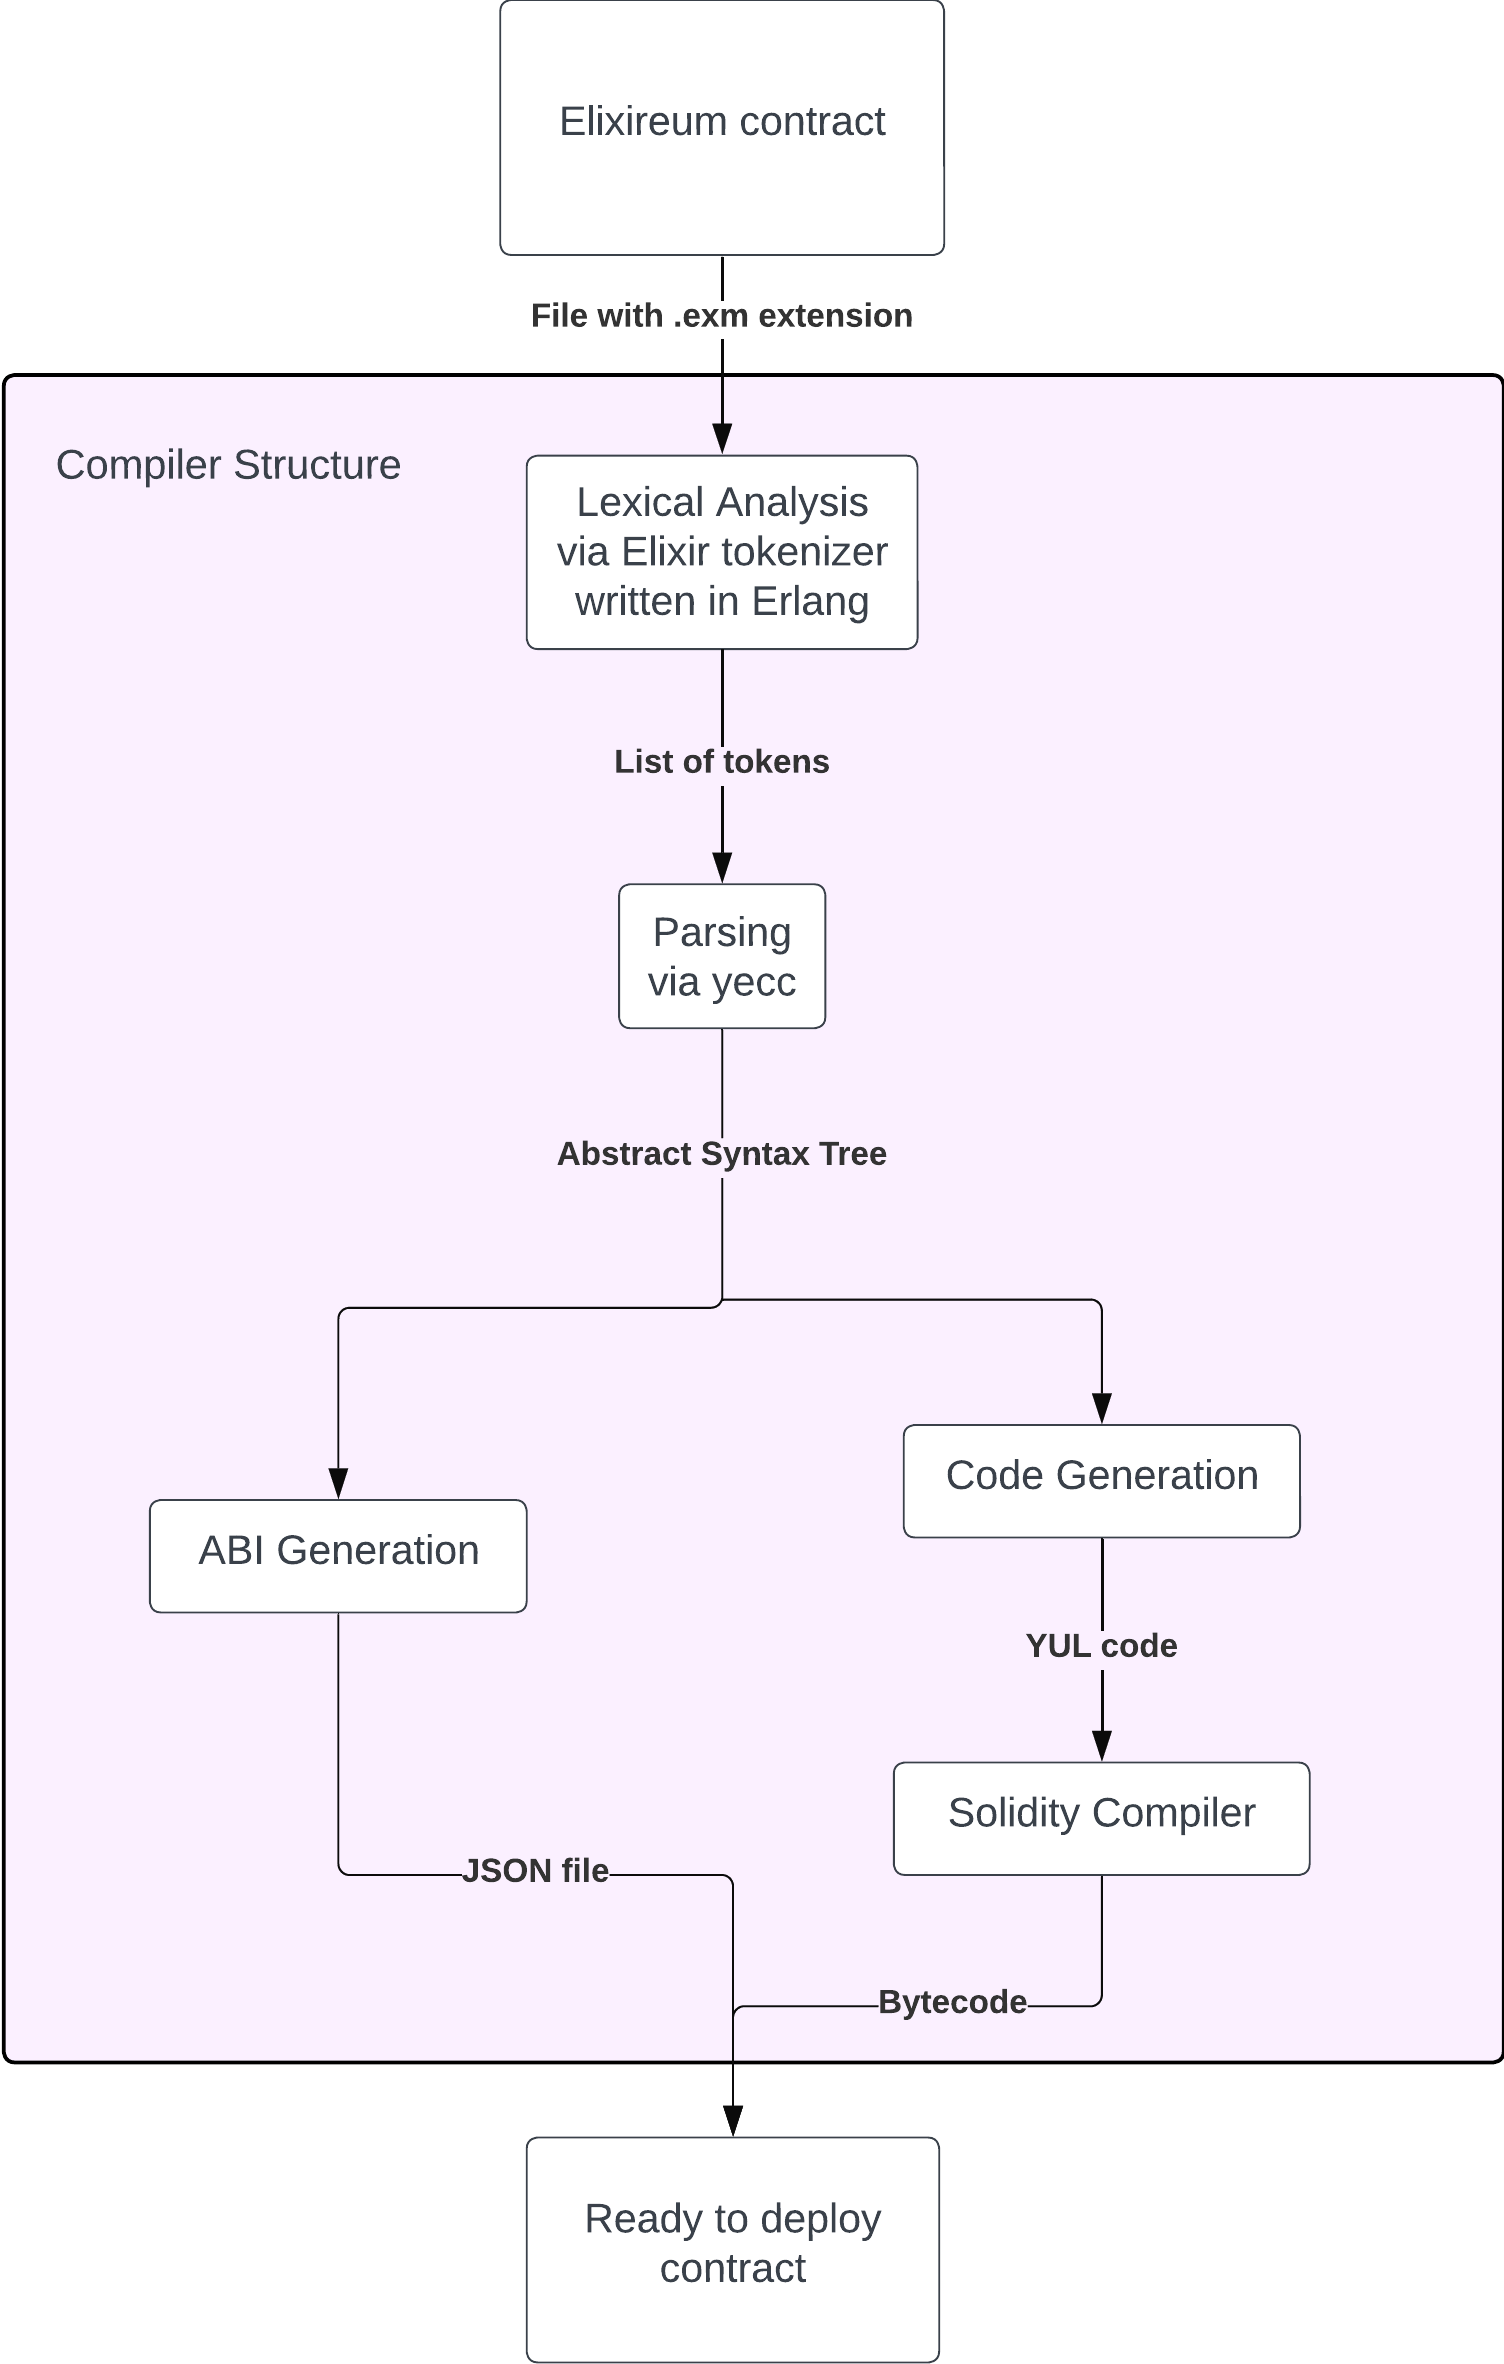
\includegraphics[width=0.8\textwidth]{figs/arch.png}
  \caption{Elixireum compiler architecture}
  \label{fig:arch}
\end{figure}

Here is the pipeline of actions performed by the main Compiler module, which can be seen visually in Fig. \ref{fig:arch}, each pipeline step is performed only if all the previous steps are successful.

\begin{itemize}
    \item Reading the source code from the file system.
    \item Running the Elixir tokenizer and parser on the source code.
    \item Performing the first pass of the Elixir AST in pre-order to gather information about defined functions, storage variables, and events, and packing this data into the following structure:
    
    \begin{lstlisting}[caption={Contract structure}, language=elixir, label={lst:contract_structure}]
      @type t :: %Contract{
          functions: Functions.t(),
          name: String.t(),
          private_functions: Functions.t(),
          variables: %{atom() => Variable.t()},
          events: %{atom() => Event.t()},
          aliases: %{atom() => list()}
        }
    \end{lstlisting}
    
    At this step, the compiler checks that public defined functions have corresponding typespecs\footnote{Typespec is the type specification of the function used in Elixir}, storage variables have types and events have all required fields.

    \item Perform the second traversal of the Elixir AST in post-order to generate Yul code.
    
    Specifically, this step generates a special function called a constructor. This function is executed at the deployment stage, and it takes its arguments not from calldata, but from the code. The Yul code that decodes arguments is generated using the calldata decoding module.

    Then, the compiler generates a function selector. The function selector is used to identify which function is being called based on the first four bytes of the call data. The first four bytes of the call data should be equal to the first four bytes of the Keccak256 hash of the string in the following format:
    \lstinline|function_name(1st_arg_type_name,2nd_arg_type_name,...)|
    constructed for the calling function, this is called method ID. For example, if the function has the following signature 
    \lstinline|transfer(address to, uint256 value)|
    Keccak256 is performed on 
    \lstinline|transfer(address,uint256)| The result of Keccak 256 is equal to 0xa9059cbb2ab0\dots So, the method ID for the transfer function is 0xa9059cbb. The function selector is simply a switch case expression where each public defined function corresponds to a case with its method ID. For each case statement, the compiler generates Yul code, responsible for function arguments decoding from call data, using the call data decoding module. Then the function call is generated as if it was a private function. Then, the compiler generates the code that encodes the value returned by the function into the return format using the return data encoding module.

    Then, the compiler generates Yul code for all user-defined functions, both public and private, since the difference between public and private functions is factored out into the function selector.

    Then, the compiler generates Yul code for standard functions used in user-defined functions. Standard functions are represented by the following structure:

    \begin{lstlisting}[caption={Standard function structure}, language=elixir, label={lst:standard_function_structure}]
      @type t :: %StdFunction{
          deps: %{atom() => t()},
          yul: String.t()
        }
    \end{lstlisting}

    The field deps represents other standard functions used by this standard function. This mechanism allows the definition of standard functions on demand, thus reducing the size of the Yul code and lowering the cost of deployment. Here is the mechanism that resolves dependencies:


    \begin{lstlisting}[caption={Standard function dependencies}, language=elixir, label={lst:standard_function_dependencies}]
    defp generate_std_functions(used_std_functions, definitions \\ %{}) do
      used_std_functions |>
      Enum.reduce(definitions, fn {function_name,
                                  %StdFunction{yul: yul, deps: deps}},
                                  definitions_acc ->
        {_, not_defined_deps} = Map.split(deps, Map.keys(definitions_acc))

        generate_std_functions(not_defined_deps, Map.put_new(definitions_acc, function_name, yul))
      end)
    end
    \end{lstlisting}
      
    
    \item Then, using the output of the first pass, the compiler generates ABI via ABI generator module.

\end{itemize}

\subsection{ABI generator}
\label{ssec:abi_generator}
The ABI generator takes the contract information collected by the compiler in the form of the contract structure \ref{lst:contract_structure} and generates a JSON ABI using the functions and events fields of the contract structure.


\subsection{Calldata decoding}
\label{ssec:calldata_decoding}
The call data decoding module recursively generates code for parsing arguments using information from the typespec of the function. The main function of this module is the decode function. It is generalized in terms of functions that perform loading and copying of data in order to reuse this function not only for argument decoding in calls, but also for argument decoding in the constructor where arguments are stored in memory, not in calldata. Here is an example of the base case of the decode function:

\begin{lstlisting}[caption={Calldata decoding base case}, language=elixir, label={lst:calldata_decoding_base}]
  def decode(
    _arg_name,
    %Type{encoded_type: encoded_type} = type,
    data_load_fn,
    _data_copy_fn,
    calldata_var,
    _init_calldata_var
  )
  when encoded_type > 69 and encoded_type < 102 do
    """
    mstore8(memory_offset$, #{type.encoded_type})
    memory_offset$ := add(memory_offset$, 1)
    mstore(memory_offset$, #{data_load_fn}(#{calldata_var}))
    memory_offset$ := add(memory_offset$, #{type.size})
    #{calldata_var} := add(#{calldata_var}, 32)
    """
  end
\end{lstlisting}

This function clause generates code that copies the value from calldata to memory and store the type for the Bytes<N> ABI type.

Here is an example of the recursive case of the decode function:

\begin{lstlisting}[caption={Calldata decoding recursive case}, language=elixir, label={lst:calldata_decoding_recursive}]
  def decode(
        arg_name,
        %Type{
          encoded_type: 3,
          components: components,
          size: size
        } = type,
        data_load_fn,
        data_copy_fn,
        calldata_var,
        init_calldata_var
      ) do
    tail_offset_var_name = "#{calldata_var}$#{arg_name}"
    init_tail_offset_var_name = "#{init_calldata_var}$#{arg_name}_init"

    """
    mstore8(memory_offset$, #{type.encoded_type})
    memory_offset$ := add(memory_offset$, 1)
    mstore(memory_offset$, #{Enum.count(components)})
    memory_offset$ := add(memory_offset$, 32)

    #{if size == :dynamic do
      """
      let #{tail_offset_var_name} := add(#{init_calldata_var}, #{data_load_fn}(#{calldata_var}))
      """
    else
      """
      let #{tail_offset_var_name} := #{calldata_var}
      """
    end}

    let #{init_tail_offset_var_name} := #{tail_offset_var_name}

    #{for {component, index} <- Enum.with_index(components) do
      decode(arg_name <> "#{index}", component, data_load_fn, data_copy_fn, tail_offset_var_name, init_tail_offset_var_name)
    end}
    """
  end
\end{lstlisting}

This function clause recursively generates code that copies the value from calldata to memory and stores type for the tuple ABI type. However, it only considers the tuple structure, i.e., the number of elements in it, and not the types of the elements, each element is decoded recursively.
  
\subsection{Emitting event}

The Event module is responsible for preparing and emitting events. Function emit, which is the main function of the module, takes the event as argument in the following form:

\begin{lstlisting}[language=elixir, caption={Event structure}, label={lst:event_structure}]
  @type t :: %Event{
          name: atom(),
          indexed_arguments: [keyword(Type.t())],
          data_arguments: [keyword(Type.t())],
          keccak256: String.t()
        }
\end{lstlisting}
  
An event has its signature, similar to a method ID for functions, but an event signature is the full Keccak256 hash of the following format:
$$event\_name(1st\_arg\_type\_name,2nd\_arg\_type\_name,...)$$

Events have indexed and data arguments. Indexed arguments are placed in the topics of the log. Topics are used to filter logs when fetching them from the blockchain. However, a log can have only up to four topics, with the first one being the event signature, so an event can have up to three indexed arguments. The size of the topics is limited to 32 bytes. For values larger than 32 bytes, its Keccak256 hash is used. The other data could be stored as data arguments that are placed in the data field of the log, with any value stored as is. The module generates code for encoding Elixireum values into indexed and data arguments. The function encode\_indexed\_argument is responsible for encoding indexed arguments. Here is the clause for types that are smaller than 32 bytes and are placed in topics as is:

\begin{lstlisting}[language=elixir, caption={Encode word-size indexed argument}, label={lst:encode_indexed_argument}]
  defp encode_indexed_argument(
    arg_name,
    %Type{encoded_type: encoded_type} = type,
    %YulNode{yul_snippet_usage: yul_snippet_usage},
    compiler_state
  )
  when encoded_type not in [1, 3, 102, 103] do
    var_name = "indexed_#{arg_name}_keccak_var$"
    arg_name_pointer = "indexed_#{arg_name}_pointer$"

    {"""
    let #{arg_name_pointer} := #{yul_snippet_usage}

    #{Utils.generate_type_check(arg_name_pointer, encoded_type, "Wrong type for indexed argument #{arg_name}", compiler_state.uniqueness_provider)}

    #{arg_name_pointer} := add(#{arg_name_pointer}, 1)
    let #{var_name} := shr(#{8 * (32 - type.size)}, mload(#{arg_name_pointer}))
    """, var_name}  
  end
\end{lstlisting}

Here is the clause for types that do not fit in one word:

\begin{lstlisting}[language=elixir, caption={Encode compex type indexed argument}, label={lst:encode_indexed_argument}]
  defp encode_indexed_argument(
         arg_name,
         %Type{} = type,
         %YulNode{yul_snippet_usage: yul_snippet_usage},
         _compiler_state
       ) do
    init_var_name = "indexed_#{arg_name}_keccak_init$"
    var_name = "indexed_#{arg_name}_keccak_var$"
    arg_name_pointer = "indexed_#{arg_name}_pointer$"

    {"""
     let #{init_var_name} := offset$
     let #{arg_name_pointer} := #{yul_snippet_usage}
     #{do_encode_indexed_argument(type, arg_name_pointer, init_var_name, 0)}
     let #{var_name} := keccak256(#{init_var_name}, sub(offset$, #{init_var_name}))
     """, var_name}
  end
\end{lstlisting}

The function do\_encode\_indexed\_argument is used to convert and copy Elixireum values to the format for Keccak256 and subsequent use in topics. It is defined recursively, similar to the calldata decode function.


The function encode\_data\_argument generates code that encodes data arguments, it uses the Return data encoding module \ref{ssec:return_data_encoding}. 

\begin{lstlisting}[language=elixir, caption={Encode data argument}, label={lst:encode_data_argument}]
  defp encode_data_argument(
         arg_name,
         %Type{} = type,
         %YulNode{yul_snippet_usage: yul_snippet_usage},
         index
       ) do
    """
    let #{arg_name}_$ := processed_return_value$
    let #{arg_name}_init$ := #{arg_name}_$
    let #{arg_name}_where_to_store_head$ := add(processed_return_value_init$, #{index * 32})
    return_value$ := #{yul_snippet_usage}
    #{Return.encode(type, "i$", "size$", "#{arg_name}_where_to_store_head$", "where_to_store_head_init$")}
    """
  end
\end{lstlisting}


\subsection{Return data encoding}
\label{ssec:return_data_encoding}

The Return data encoding module is responsible for encoding the value returned by an Elixireum function to an ABI format according to the typespec. It uses a similar approach to the calldata decoding module, but in the opposite way. The main function of this module is encode. Here is the base case of this function for simple types:

\begin{lstlisting}[language=elixir, caption={Encode base case}, label={lst:encode_base_case}]
  def encode(
    %Type{encoded_type: encoded_type, size: byte_size},
    _i_var_name,
    _size_var_name,
    where_to_store_head_var_name,
    _where_to_store_head_init_var_name
  )
  when encoded_type > 69 and encoded_type < 102 do
    offset = 8 * (32 - byte_size)

    """
    #{Utils.generate_type_check(...)}

    return_value$ := add(return_value$, 1)

    mstore(#{where_to_store_head_var_name}, shl(#{offset}, shr(#{offset}, mload(return_value$))))
    #{where_to_store_head_var_name} := add(#{where_to_store_head_var_name}, 32)

    return_value$ := add(return_value$, #{byte_size})
    """
  end
\end{lstlisting}

Here is an example of a recursive case:

\begin{lstlisting}[language=elixir, caption={Encode recursive case}, label={lst:encode_recursive_case}]
  def encode(
        %Type{
          encoded_type: 103 = encoded_type,
          items_count: size,
          components: [components]
        },
        i_var_name,
        size_var_name,
        where_to_store_head_var_name,
        where_to_store_head_init_var_name
      )
      when is_integer(size) do
    """
    #{Utils.generate_type_check(...)}

    return_value$ := add(return_value$, 1)
    let #{size_var_name} := mload(return_value$)

    #{Utils.generate_value_check(...)}

    return_value$ := add(return_value$, 32)

    for { let #{i_var_name} := 0 } lt(#{i_var_name}, #{size_var_name}) { #{i_var_name} := add(#{i_var_name}, 1) } {
      #{encode(components, i_var_name <> "_", size_var_name <> "_", where_to_store_head_var_name, where_to_store_head_init_var_name)}
    }
    """
  end
\end{lstlisting}
    
\chapter{Results and Discussion}
\label{chap:res}


% 0. What/Why(purpose) Metrics 
%   - gas consumption
%     - on deploy
%     - on interacting
%   - compilation time
%   - ram/cpu usage at compilation time

% 1. test suite description (sources)

% \begin{lstlisting}[caption={ERC-20.exm}, language=elixir]
% defmodule ERC20 do
% ...
% end
% \end{lstlisting}

% \begin{lstlisting}[caption={ERC-721.exm}, language=elixir]
% defmodule ERC721 do
% ...
% end
% \end{lstlisting}

    
% 2. tests structure description
% - test suit works for all aforementioned contracts
%   - contract successfully compiles to EVM bytecode
%   - bytecode successfully deploys
%   - deployed contracts passes unit tests
% - gas consumption measurements
%     - on deploy
%     - on interacting
% - compilation time measurements
% - ram/cpu usage at compilation time measurements
% 3. test/metrics results one by one
% 4. results and comparison with Solidity
% 5. Discussion

% \subsection{Performance Metrics}
% Performance testing focuses on quantifying:
% \begin{enumerate}
%     \item \textbf{Gas Consumption}: Measured during both the deployment phase and subsequent contract interactions, providing insights into the cost efficiency of using Elixireum.
%     \item \textbf{Compilation Time}: The duration taken to compile contracts to bytecode, indicative of the compiler's efficiency.
%     \item \textbf{RAM/CPU Usage}: Monitored during the compilation process, reflecting the resource demands of the Elixireum compiler.
% \end{enumerate}

% This structured approach ensures a thorough evaluation of Elixireum, highlighting its capabilities and identifying areas for improvement. The subsequent section presents a detailed comparison of the test results, contrasting Elixireum's performance with Solidity to underscore its potential benefits and limitations.

This chapter presents an overview of results. Section \ref{sec:results_and_comparison} provides results we got during assessment of the Elixireum. Section \ref{sec:discussion} contains an interpretation of results.

\section{Results and Comparison}
\label{sec:results_and_comparison}
We conducted a series of tests by applying the test suite to a set of prepared smart contracts. All tests concluded successfully, signifying the achievement of the main project goal: a compiler capable of translating Elixireum language into EVM bytecode is developed. Moreover we deployed an ERC-20 token implemented in Elixireum to Sepolia testnet, the following hex bytes is the address of the deployed token 0x9DC699F6F8F3E42D4C6ae368C751325dC4106279\footnote{\url{https://eth-sepolia.blockscout.com/token/0x9dc699f6f8f3e42d4c6ae368c751325dc4106279}}. We then proceeded to compare Elixireum with Solidity. We benchmarked the public functions of the ERC-20 implementation in Elixireum and its full analogue in Solidity, and conducted the same benchmarking for the ERC-721 implementation. Tables~\ref{tab:erc20_comparison} and \ref{tab:erc721_comparison} present the detailed metrics that we obtained.


\begin{table}[h!]
\centering
\renewcommand{\arraystretch}{1.2}
\begin{tabular}{|c|c|c|}
\hline
\textbf{Method} & \textbf{Elixireum Gas Used} & \textbf{Solidity Gas Used} \\ \hline
mint            & 58197.4              & 54799.6              \\ \hline
approve         & 47619.8              & 46570.8              \\ \hline
transferFrom    & 54812.0              & 48492.2              \\ \hline
transfer        & 55659.8              & 51813.4              \\ \hline
burn            & 33061.6              & 29433.25             \\ \hline
deploy of contract       & 1939441              & 732543               \\ \hline
\end{tabular}
\caption{ERC-20 contract gas usage comparison (20 runs)}
\label{tab:erc20_comparison}
\end{table}

\begin{table}[h!]
\centering
\renewcommand{\arraystretch}{1.2}
\begin{tabular}{|c|c|c|}
\hline
\textbf{Method}         & \textbf{Elixireum Gas Used} & \textbf{Solidity Gas Used} \\ \hline
setApprovalForAll       & 46596.0              & 46304.0              \\ \hline
mint                    & 166817.4             & 162675.4             \\ \hline
transferFrom            & 87123.0              & 55652.6              \\ \hline
approve                 & 54798.0              & 49007.8              \\ \hline
burn                    & 58539.6              & 29944.0              \\ \hline
deploy of contract                 & 3067454              & 1113786              \\ \hline
\end{tabular}
\caption{ERC-721 contract gas usage comparison (20 runs)}
\label{tab:erc721_comparison}
\end{table}

  The comparison reveals that while Elixireum successfully implements the functionalities of ERC-20 and ERC-721 contracts, it generally consumes more gas compared to Solidity for the same operations. Table~\ref{tab:erc20_comparison} shows that, on average, Elixireum is 8\% less efficient than Solidity for function calls of ERC-20 methods and approximately 164\% less efficient in terms of gas consumption during the deployment process. Table~\ref{tab:erc721_comparison} indicates even less favorable metrics: Elixireum is about 20.5\% less efficient for ERC-721 methods and consumes 175\% more gas during deployment. These findings indicate that while Elixireum is functional and compatible with the Ethereum blockchain, there is a need for optimization to reduce gas consumption and improve efficiency.

\section{Discussion}
\label{sec:discussion}

The findings from this chapter contribute significantly to the broader thesis goal of assessing the feasibility and potential of Elixireum in the context of smart contract development. We confirmed our hypothesis that an Elixir-like language can be compiled to EVM.

Moreover, we conducted a comprehensive comparison of gas consumption between Elixireum and Solidity. While the results showed that Elixireum consumes 2.7 times more gas than Solidity for deployment, the gas usage for ERC-20 and ERC-721 methods is comparable. This demonstrates that it is possible to have a functional language with dynamic typing and types stored in memory that consumes approximately 14\% more gas than Solidity.

With the rise of rollup chains mentioned in Chapter \ref{chap:intro}, the tradeoff between gas consumption and development ease should be considered. While a call of contract written with Elixireum may cost \$1.15 instead of \$1 with Solidity due to higher gas consumption, the ease and speed of development with Elixireum can lead to earlier deployment. This earlier deployment can attract more users, potentially outweighing the slight increase in gas costs.


\printbibliography[heading=bibintoc,title={Список использованной литературы}]
\end{document}

